\begin{frame}{POO: El Objeto}
\justifying
\begin{itemize}
\item Un objeto es una unidad que engloba en sí mismo características y comportamiento necesario para procesar infomración. Cada objeto contiene datos y funciones. Y un programa se construye como un objeto de objetos, o como un único objeto.
\end{itemize}
{\tiny Python Manizales - Jesse Padilla Agudelo}
\end{frame}

\begin{frame}{POO: El Objeto}
\justifying
Ejemplo:
\begin{itemize}
\item Carro BMW.\\
Características:
	\begin{itemize}
	\item 4 ruedas 	Michelline.
	\item Motor BMW.
	\item Caja de cambios de 7 velocidades.
	\item Color Azul.
	\item 2 espejos.
	\end{itemize}
\end{itemize}
{\tiny Python Manizales - Jesse Padilla Agudelo}
\end{frame}

\begin{frame}{POO: La Clase}
\justifying
La clase es un modelo o prototipo que define las variables y métodos comunes a todos los objetos de cierta clase. También se puede decir que una clase es una plantilla genérica para un conjunto de objetos de similares características.

{\tiny Python Manizales - Jesse Padilla Agudelo}
\end{frame}

\begin{frame}{POO: La Clase}
\justifying

Ejemplo:
\begin{itemize}
\item Carro Vehículo.
	\begin{itemize}
	\item Número de ruedas.
	\item Tipo de Motor.
	\item Capacidad del tanque de gasolina.
	\item Número de velocidades de la caja de cambios.
	\item Color.
	\end{itemize}
\end{itemize}

{\tiny Python Manizales - Jesse Padilla Agudelo}
\end{frame}

\begin{frame}{POO: El Mensaje}
\justifying
\begin{itemize}
\item El mensaje es el modo en que se comunican los objetos entre si.\\
Ejemplo:
\begin{itemize}
\item Cuando llamemos a una función de un objeto, diremos que estamos enviando un mensaje a ese objeto.
\end{itemize}
\end{itemize}
{\tiny Python Manizales - Jesse Padilla Agudelo}
\end{frame}

\begin{frame}{POO: El Objeto}
\justifying
\begin{figure}[H]
\centering
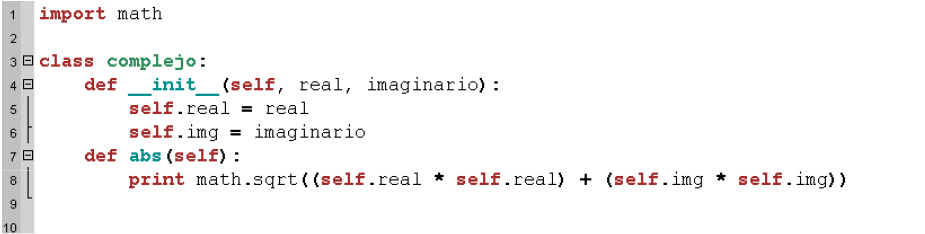
\includegraphics[scale=0.35]{Section_Files/images/02.png}
\caption{Interfaz del Anaconda Navigator.}
\end{figure}
{\tiny Python Manizales - Jesse Padilla Agudelo}
\end{frame}

